
In this chapter, we propose two new methods for estimating any sample quantile $\theta_q$ of the true extinction date, given a set of fossils. Both of these methods use test-statistic inversion: we first describe a novel approach called MINMI, which directly inverts a minimum statistic to estimate a quantile; then we describe an application of the \citet{Garthwaite1992} implementation of the Robbins-Monro process for generating Monte Carlo confidence intervals via inversion. 

\section{Minimum-Statistic Inversion (MINMI) Estimator}\label{new-method}

The MINMI\footnote{The name MINMI is a reference to \textit{Minmi}, a genus of ankylosaur (or armoured dinosaur). Notably, \textit{Minmi} is the only known genus of ankylosaur from Australia \cite{Carpenter2001}} estimator assumes fossil recovery is uniformly distributed and that the distribution of measurement errors is known with constant variance. Then, using these assumptions, we are able to directly construct a quantile estimator by inversion. Recall that we have observed fossil dates (measured in calibrated years before present) $W_1, W_2, \dots, W_n$ such that:
\[
W_i = X_i + \varepsilon_i, \quad i = 1, 2, \dots, n
\]
where $X_i$ are the unobserved fossil dates such that $X_i | \varepsilon_i \sim \mathcal{U}(\theta, K - e_i)$; $\varepsilon_i$ come from a known distribution $f_{\varepsilon}$ independent to $X_i$; and $\varepsilon_i$ are i.i.d $\forall i$ with $\E[\varepsilon_i] = 0$ and $\Var(\varepsilon_i) = \sigma^2$ and we further condition on $\varepsilon_i<K=\theta$.

\subsection{No Measurement Error Scenario}

If we assume measurement error is negligible, we may completely eliminate $\varepsilon$ from the above. Thus, the quantile estimate becomes trivial to find as the joint density of $(X, \varepsilon)$ is equivalent to the density of $X$, a uniformly distributed random variable on the interval $[\theta, K]$. Let the test statistic $S(\bm{W})$ be the minimum statistic (which is the maximum likelihood estimator in this scenario), and let $m$ denote the observed minimum value of $S(\bm{W})$:
\begin{align*}
    \PP_\theta (S(\bm{W}) \geq m)
        &= \prod_{i=1}^n \PP_\theta (X_i \geq m) \\
        &= \left[ \PP_\theta (X_i \geq m) \right]^n, \quad \text{since our $X$'s are assumed i.i.d}\\
        &= \left( \frac{K - m}{K - \theta} \right)^n
\end{align*}

Applying test-statistic inversion as per \autoref{eq: inversion}, we have
\begin{align*}\label{eq:minmi-no-measurement-error}
    q &= \PP_{\hat{\theta}_q}(M \geq m) = \left( \frac{K - m}{K - \hat{\theta}_q} \right)^n \\
    \therefore \hat{\theta}_q &= K - q^{-1/n} (K-m) \numberthis
\end{align*}

where $\hat\theta_q$ is the MINMI estimate of $\theta_q$, the $q\textsuperscript{th}$ sample quantile of $\theta$, such that $\PP_{\theta_q} (S(\bm{W}) \geq m) = q$.

\subsection{Measurement Error Scenario}

Suppose we do in fact have measurement error. Then, we must first consider the joint density of $(X, \varepsilon)$, which is \[ f_{X, \varepsilon} ( x , \varepsilon) = c f_{X | \varepsilon} ( x | \varepsilon=e) f_\varepsilon(e) \]

where $x > \theta$, $x+e \leq K$, and $c$ is a normalising constant. Rearranging to find $c$:
\begin{align*}
    c^{-1}
        &= \int_{e=-\infty}^{K-\theta} \int_{x=\theta}^{K-e} f_{X | \varepsilon} ( x | \varepsilon=e) f_\varepsilon(e) dx de = \int_{e=-\infty}^{K-\theta} f_\varepsilon(e) de \\
    \therefore c^{-1} &= F_\varepsilon(K - \theta)
\end{align*}

Thus our joint density function is given by \begin{align*}
    f_{X, \varepsilon} ( x , \varepsilon)
        =& [F_\varepsilon(K - \theta)]^{-1} f_{X | \varepsilon} ( x | \varepsilon=e) f_\varepsilon(e) \\
        =& [F_\varepsilon(K - \theta)]^{-1} \frac{1}{K - e - \theta} f_\varepsilon(e)
\end{align*}

since $f_{X | \varepsilon} ( x | \varepsilon=e) = \frac{1}{K - e - \theta}$ ($X|\varepsilon$ is conditionally uniform). 

From this, we can geometrically identify our region of interest as shown by the shaded region of \autoref{fig: minmi_integral}.
\begin{figure}[ht]
    \centering
    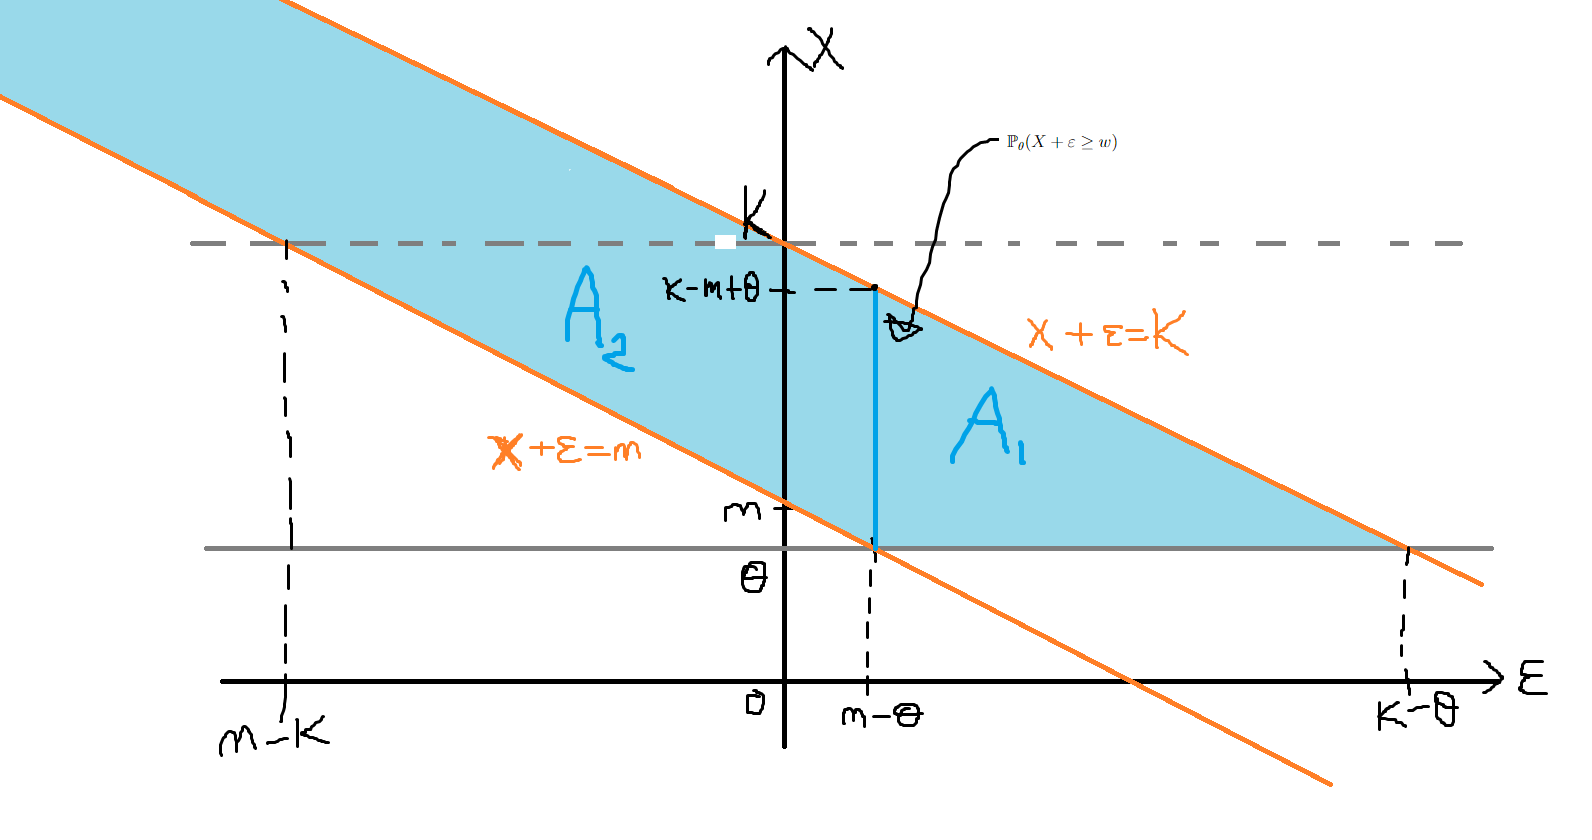
\includegraphics[width=0.8\textwidth]{figures/minmi-integral-sketch.png}
    \caption{Sketch of the region of the joint density $(X, \varepsilon)$, indicated by the shaded area. Note that it is bounded by the lines $X+\varepsilon = K$ and $X + \varepsilon = m$, and that the measurement errors are truncated at $K-\theta$.}
    \label{fig: minmi_integral}
\end{figure}

Hence, we can find $\PP_\theta ( X + \varepsilon \geq w)$ for some value $w$. \begin{align*}
    \PP_\theta ( X + \varepsilon \geq w)
        =& 1 - \PP_\theta ( X + \varepsilon < w) \\
        =& 1 - \int_{-\infty}^{w-\theta} \int_{\theta}^{w-e} f_{X, \varepsilon}(x, e) dx de \quad \text{by inspection} \\
        =& 1 - \int_{-\infty}^{w-\theta} \int_{\theta}^{w-e} \frac{1}{K - \theta - e} \frac{1}{F_\varepsilon (K - \theta)} f_\varepsilon(e) dx de \\
        =& 1 - \frac{1}{F_\varepsilon (K-\theta)} \int_{-\infty}^{w-\theta} \frac{w - \theta - e }{K - \theta - e} f_\varepsilon(e) de \\
    \therefore \PP_\theta ( X + \varepsilon \geq w) =& 1 - \frac{F_\varepsilon(w-\theta)}{F_\varepsilon(K - \theta)} \psi(\theta; w) \numberthis \label{eqn:minmi}
\end{align*} where 
\[
 \psi(\theta; w) =  \int^{w-\theta}_{-\infty} \frac{w - e - \theta}{K - e - \theta) } \frac{f_\varepsilon(e)}{F_\varepsilon(w-\theta)} de
\]

As before, we let our statistic $S(\bm{W})$ be the minimum statistic, $m$ be the observed minimum, and $\theta_q$ be the $q\textsuperscript{th}$ quantile such that $\PP_{\theta_q} (S(\bm{W}) \geq m) = q$: \begin{align*}
    q &= \PP_{\theta_q} (S(\bm{W}) \geq m) \\
        &= \prod_{i=1}^n \PP_{\theta_q} (X_{i} + \varepsilon_i \geq m) \\
        &= \left[ 1 - \frac{F_\varepsilon(m-\theta_q)}{F_\varepsilon(K - \theta_q)} \psi(\theta_q; m)  \right]^n \\
    q^{\frac{1}{n}} &= 1 - \frac{F_\varepsilon(m-\theta_q)}{F_\varepsilon(K - \theta_q)} \psi(\theta_q; m) \numberthis \label{eqn: minmi-ee}
\end{align*}

The MINMI estimator $\hat\theta_q$ can be found using inversion by solving the above equation for $\theta = \hat\theta_q$. However, since $\psi$ does not simplify in general, we can approximate it with a Monte Carlo integral using $B$ samples, resulting in the below MINMI estimating equation: \begin{align*}
    q^{\frac{1}{n}} &= 1 - \frac{F_\varepsilon(m - \theta_q)}{F_\varepsilon(K - \theta_q)} \hat\psi_B(\theta_q; m); &\hat\psi_B(\theta_q; m) =  \frac{1}{B} \sum_{b=1}^B \frac{m-e_b-\hat\theta_q}{K-e_b-\theta_q} \numberthis \label{eqn: minmi-ee-mc}
\end{align*}

where $e_b$ are drawn from $f_\varepsilon(e_b)$ truncated at $m-\hat\theta_q$

\subsection{Stochastically Increasing Property}

Generating confidence intervals by inversion is conditional on $\PP_{\theta_q} (S(\bm{W}) \geq m)$ being stochastically increasing in $\theta$. Although we were unable to show theoretically that this condition is true in general for any density function $f$ and all values of $\varepsilon$, we were able to simplify this assumption to be true according two some constraints, which we believe to be reasonable to assume. We were also able to show numerically that, under the assumption of normally distributed errors $\varepsilon$, $\PP_{\theta_q} (S(\bm{W}) \geq m)$ is indeed stochastically increasing in $\theta$. The working out used to simplify this assumption to the constraints has been provided in \autoref{apx:minmi-stoch-incr-proof}.

\subsection{Selecting the number of Monte Carlo Samples}

There is a question of how large $B$ needs to ``be". As the number of Monte Carlo samples increases, the variance of the MINMI estimator can be expected to decrease: however, we would like to determine a way to obtain a ``good" value for $B$ since a large $B$ would result in estimates with low variance of Monte Carlo error at the cost of more computation. Using the delta method, we were able to show how the Monte Carlo error changes as $B \rightarrow \infty$.

\begin{theorem}\label{eqn:minmi_mce}
    The limiting distribution of the MINMI estimator $\hat\theta_q$ of the q\textsuperscript{th} sample quantile $\theta_q$ as $B \rightarrow \infty$ is approximately normal, where $B$ is the number of Monte Carlo samples used.
    $$\sqrt{B}(\hat\theta_q - \theta_q) \sim \cN \left(0, \sigma^2_{\psi(\theta_q)} \left[ \frac{F(m-\theta_q)}{F(K-\theta_q)\hat{u}^\prime(\theta_q)} \right]^2 \right)$$
\end{theorem}
A full derivation of this result is given in \autoref{apx:minmi-asymptotics-proof}.

In practice, we are interested in values of $B$ that result in ``low" variance estimates. To do so, we can use the following equation \[
B \approx \frac{\sigma^2_{\psi(\theta_q)}}{\Var{\hat\theta_q}} \left[ \frac{F(m-\theta_q)}{F(K-\theta_q)\hat{u}^\prime(\theta_q)} \right]^2
\] where $\sigma^2_{\theta_q}$ is some ``small" amount of variance we are comfortable with.

Note that the true values for $\theta_q$ and $\sigma^2_{\psi(\theta_q)}$ will usually be unknown. For our purposes, pilot estimates would suffice for obtaining a value of $B$ that gives estimates with Monte Carlo error roughly equal to $\Var \hat\theta_q^*$. For instance, a pilot estimate of $\theta_q$ can be obtained using the no-measurement error scenario proposed i \autoref{eq:minmi-no-measurement-error}, and a Monte Carlo estimate of $\sigma^2_{\psi(\theta_q)}$ can be obtained using some pilot number of Monte Carlo samples, such as $B=500$.

We were also able to verify these results numerically, comparing the variance estimated by \autoref{eqn:minmi_mce} to the sample variance from 1000 estimates for the upper and lower endpoints of a central $95\%$ confidence interval at different values of $B$. Since this is a delta method approximation of the variance, it relies on an assumption that the estimating equation (\autoref{eqn: minmi-ee-u(theta)}) is approximately linear in $\theta_q$. This assumption is only reasonable at large values of $B$, which we observed to be accurate to within \textcolor{red}{XXX\% for $B > 500$ (See Figure YYY). Since we are using this to \textit{guide} the choice of $B$, this degree of accuracy is acceptable in practice.}

% \begin{figure}[ht]
%     \centering
%     % Created by tikzDevice version 0.12.3.1 on 2022-10-23 13:48:12
% !TEX encoding = UTF-8 Unicode
\begin{tikzpicture}[x=1pt,y=1pt]
\definecolor{fillColor}{RGB}{255,255,255}
\path[use as bounding box,fill=fillColor,fill opacity=0.00] (0,0) rectangle (505.89,505.89);
\begin{scope}
\path[clip] ( 49.20, 61.20) rectangle (480.69,456.69);
\definecolor{drawColor}{RGB}{0,0,255}

\path[draw=drawColor,line width= 0.4pt,line join=round,line cap=round] ( 71.14,247.56) -- ( 79.93,246.51);

\path[draw=drawColor,line width= 0.4pt,line join=round,line cap=round] ( 86.94,239.89) -- ( 99.53,169.12);

\path[draw=drawColor,line width= 0.4pt,line join=round,line cap=round] (103.89,168.22) -- (108.65,175.39);

\path[draw=drawColor,line width= 0.4pt,line join=round,line cap=round] (112.36,186.37) -- (128.76,436.06);

\path[draw=drawColor,line width= 0.4pt,line join=round,line cap=round] (130.34,436.16) -- (134.78,414.24);

\path[draw=drawColor,line width= 0.4pt,line join=round,line cap=round] (137.56,402.57) -- (145.78,372.68);

\path[draw=drawColor,line width= 0.4pt,line join=round,line cap=round] (150.53,371.99) -- (153.51,376.77);

\path[draw=drawColor,line width= 0.4pt,line join=round,line cap=round] (159.15,376.40) -- (165.60,362.15);

\path[draw=drawColor,line width= 0.4pt,line join=round,line cap=round] (169.96,350.99) -- (175.50,334.25);

\path[draw=drawColor,line width= 0.4pt,line join=round,line cap=round] (179.07,322.80) -- (185.94,299.46);

\path[draw=drawColor,line width= 0.4pt,line join=round,line cap=round] (188.29,299.66) -- (197.43,382.26);

\path[draw=drawColor,line width= 0.4pt,line join=round,line cap=round] (209.56,376.35) -- (218.19,334.99);

\path[draw=drawColor,line width= 0.4pt,line join=round,line cap=round] (221.71,323.57) -- (227.25,310.19);

\path[draw=drawColor,line width= 0.4pt,line join=round,line cap=round] (234.38,308.20) -- (234.87,308.56);

\path[draw=drawColor,line width= 0.4pt,line join=round,line cap=round] (243.01,307.12) -- (246.26,302.18);

\path[draw=drawColor,line width= 0.4pt,line join=round,line cap=round] (250.85,303.04) -- (258.28,337.09);

\path[draw=drawColor,line width= 0.4pt,line join=round,line cap=round] (261.81,348.51) -- (268.03,363.94);

\path[draw=drawColor,line width= 0.4pt,line join=round,line cap=round] (272.54,363.95) -- (278.00,350.61);

\path[draw=drawColor,line width= 0.4pt,line join=round,line cap=round] (283.82,349.90) -- (286.97,354.19);

\path[draw=drawColor,line width= 0.4pt,line join=round,line cap=round] (294.37,363.62) -- (297.00,366.76);

\path[draw=drawColor,line width= 0.4pt,line join=round,line cap=round] (312.70,379.67) -- (319.63,404.93);

\path[draw=drawColor,line width= 0.4pt,line join=round,line cap=round] (323.19,405.05) -- (329.50,386.98);

\path[draw=drawColor,line width= 0.4pt,line join=round,line cap=round] (335.99,377.37) -- (337.24,376.28);

\path[draw=drawColor,line width= 0.4pt,line join=round,line cap=round] (343.50,366.59) -- (350.24,344.55);

\path[draw=drawColor,line width= 0.4pt,line join=round,line cap=round] (367.16,338.52) -- (367.66,338.89);

\path[draw=drawColor,line width= 0.4pt,line join=round,line cap=round] (387.65,345.19) -- (388.14,345.55);

\path[draw=drawColor,line width= 0.4pt,line join=round,line cap=round] (395.04,354.70) -- (401.20,371.88);

\path[draw=drawColor,line width= 0.4pt,line join=round,line cap=round] (406.93,382.26) -- (409.80,385.93);

\path[draw=drawColor,line width= 0.4pt,line join=round,line cap=round] (427.23,395.26) -- (430.48,399.79);

\path[draw=drawColor,line width= 0.4pt,line join=round,line cap=round] (439.00,401.38) -- (439.19,401.25);

\path[draw=drawColor,line width= 0.4pt,line join=round,line cap=round] (445.32,392.07) -- (453.35,349.33);

\path[draw=drawColor,line width= 0.4pt,line join=round,line cap=round] (456.23,349.17) -- (462.95,371.04);

\path[draw=drawColor,line width= 0.4pt,line join=round,line cap=round] ( 65.18,248.27) circle (  2.25);

\path[draw=drawColor,line width= 0.4pt,line join=round,line cap=round] ( 85.89,245.79) circle (  2.25);

\path[draw=drawColor,line width= 0.4pt,line join=round,line cap=round] (100.58,163.22) circle (  2.25);

\path[draw=drawColor,line width= 0.4pt,line join=round,line cap=round] (111.97,180.38) circle (  2.25);

\path[draw=drawColor,line width= 0.4pt,line join=round,line cap=round] (129.15,442.04) circle (  2.25);

\path[draw=drawColor,line width= 0.4pt,line join=round,line cap=round] (135.97,408.36) circle (  2.25);

\path[draw=drawColor,line width= 0.4pt,line join=round,line cap=round] (147.37,366.90) circle (  2.25);

\path[draw=drawColor,line width= 0.4pt,line join=round,line cap=round] (156.68,381.87) circle (  2.25);

\path[draw=drawColor,line width= 0.4pt,line join=round,line cap=round] (168.07,356.69) circle (  2.25);

\path[draw=drawColor,line width= 0.4pt,line join=round,line cap=round] (177.38,328.56) circle (  2.25);

\path[draw=drawColor,line width= 0.4pt,line join=round,line cap=round] (187.63,293.70) circle (  2.25);

\path[draw=drawColor,line width= 0.4pt,line join=round,line cap=round] (198.09,388.23) circle (  2.25);

\path[draw=drawColor,line width= 0.4pt,line join=round,line cap=round] (208.33,382.23) circle (  2.25);

\path[draw=drawColor,line width= 0.4pt,line join=round,line cap=round] (219.42,329.12) circle (  2.25);

\path[draw=drawColor,line width= 0.4pt,line join=round,line cap=round] (229.55,304.64) circle (  2.25);

\path[draw=drawColor,line width= 0.4pt,line join=round,line cap=round] (239.70,312.12) circle (  2.25);

\path[draw=drawColor,line width= 0.4pt,line join=round,line cap=round] (249.57,297.17) circle (  2.25);

\path[draw=drawColor,line width= 0.4pt,line join=round,line cap=round] (259.56,342.95) circle (  2.25);

\path[draw=drawColor,line width= 0.4pt,line join=round,line cap=round] (270.27,369.51) circle (  2.25);

\path[draw=drawColor,line width= 0.4pt,line join=round,line cap=round] (280.27,345.06) circle (  2.25);

\path[draw=drawColor,line width= 0.4pt,line join=round,line cap=round] (290.52,359.02) circle (  2.25);

\path[draw=drawColor,line width= 0.4pt,line join=round,line cap=round] (300.85,371.36) circle (  2.25);

\path[draw=drawColor,line width= 0.4pt,line join=round,line cap=round] (311.12,373.89) circle (  2.25);

\path[draw=drawColor,line width= 0.4pt,line join=round,line cap=round] (321.21,410.72) circle (  2.25);

\path[draw=drawColor,line width= 0.4pt,line join=round,line cap=round] (331.48,381.32) circle (  2.25);

\path[draw=drawColor,line width= 0.4pt,line join=round,line cap=round] (341.75,372.32) circle (  2.25);

\path[draw=drawColor,line width= 0.4pt,line join=round,line cap=round] (352.00,338.82) circle (  2.25);

\path[draw=drawColor,line width= 0.4pt,line join=round,line cap=round] (362.30,335.00) circle (  2.25);

\path[draw=drawColor,line width= 0.4pt,line join=round,line cap=round] (372.52,342.41) circle (  2.25);

\path[draw=drawColor,line width= 0.4pt,line join=round,line cap=round] (382.78,341.69) circle (  2.25);

\path[draw=drawColor,line width= 0.4pt,line join=round,line cap=round] (393.01,349.05) circle (  2.25);

\path[draw=drawColor,line width= 0.4pt,line join=round,line cap=round] (403.23,377.53) circle (  2.25);

\path[draw=drawColor,line width= 0.4pt,line join=round,line cap=round] (413.49,390.66) circle (  2.25);

\path[draw=drawColor,line width= 0.4pt,line join=round,line cap=round] (423.73,390.39) circle (  2.25);

\path[draw=drawColor,line width= 0.4pt,line join=round,line cap=round] (433.98,404.66) circle (  2.25);

\path[draw=drawColor,line width= 0.4pt,line join=round,line cap=round] (444.21,397.97) circle (  2.25);

\path[draw=drawColor,line width= 0.4pt,line join=round,line cap=round] (454.46,343.44) circle (  2.25);

\path[draw=drawColor,line width= 0.4pt,line join=round,line cap=round] (464.71,376.77) circle (  2.25);
\end{scope}
\begin{scope}
\path[clip] (  0.00,  0.00) rectangle (505.89,505.89);
\definecolor{drawColor}{RGB}{0,0,0}

\path[draw=drawColor,line width= 0.4pt,line join=round,line cap=round] ( 65.18, 61.20) -- (464.71, 61.20);

\path[draw=drawColor,line width= 0.4pt,line join=round,line cap=round] ( 65.18, 61.20) -- ( 65.18, 55.20);

\path[draw=drawColor,line width= 0.4pt,line join=round,line cap=round] (111.97, 61.20) -- (111.97, 55.20);

\path[draw=drawColor,line width= 0.4pt,line join=round,line cap=round] (147.37, 61.20) -- (147.37, 55.20);

\path[draw=drawColor,line width= 0.4pt,line join=round,line cap=round] (182.76, 61.20) -- (182.76, 55.20);

\path[draw=drawColor,line width= 0.4pt,line join=round,line cap=round] (229.55, 61.20) -- (229.55, 55.20);

\path[draw=drawColor,line width= 0.4pt,line join=round,line cap=round] (264.94, 61.20) -- (264.94, 55.20);

\path[draw=drawColor,line width= 0.4pt,line join=round,line cap=round] (300.34, 61.20) -- (300.34, 55.20);

\path[draw=drawColor,line width= 0.4pt,line join=round,line cap=round] (347.13, 61.20) -- (347.13, 55.20);

\path[draw=drawColor,line width= 0.4pt,line join=round,line cap=round] (382.52, 61.20) -- (382.52, 55.20);

\path[draw=drawColor,line width= 0.4pt,line join=round,line cap=round] (417.92, 61.20) -- (417.92, 55.20);

\path[draw=drawColor,line width= 0.4pt,line join=round,line cap=round] (464.71, 61.20) -- (464.71, 55.20);

\node[text=drawColor,anchor=base,inner sep=0pt, outer sep=0pt, scale=  1.00] at ( 65.18, 39.60) {2};

\node[text=drawColor,anchor=base,inner sep=0pt, outer sep=0pt, scale=  1.00] at (111.97, 39.60) {5};

\node[text=drawColor,anchor=base,inner sep=0pt, outer sep=0pt, scale=  1.00] at (147.37, 39.60) {10};

\node[text=drawColor,anchor=base,inner sep=0pt, outer sep=0pt, scale=  1.00] at (182.76, 39.60) {20};

\node[text=drawColor,anchor=base,inner sep=0pt, outer sep=0pt, scale=  1.00] at (229.55, 39.60) {50};

\node[text=drawColor,anchor=base,inner sep=0pt, outer sep=0pt, scale=  1.00] at (264.94, 39.60) {100};

\node[text=drawColor,anchor=base,inner sep=0pt, outer sep=0pt, scale=  1.00] at (300.34, 39.60) {200};

\node[text=drawColor,anchor=base,inner sep=0pt, outer sep=0pt, scale=  1.00] at (347.13, 39.60) {500};

\node[text=drawColor,anchor=base,inner sep=0pt, outer sep=0pt, scale=  1.00] at (382.52, 39.60) {1000};

\node[text=drawColor,anchor=base,inner sep=0pt, outer sep=0pt, scale=  1.00] at (417.92, 39.60) {2000};

\node[text=drawColor,anchor=base,inner sep=0pt, outer sep=0pt, scale=  1.00] at (464.71, 39.60) {5000};

\path[draw=drawColor,line width= 0.4pt,line join=round,line cap=round] ( 49.20,123.74) -- ( 49.20,447.49);

\path[draw=drawColor,line width= 0.4pt,line join=round,line cap=round] ( 49.20,123.74) -- ( 43.20,123.74);

\path[draw=drawColor,line width= 0.4pt,line join=round,line cap=round] ( 49.20,188.49) -- ( 43.20,188.49);

\path[draw=drawColor,line width= 0.4pt,line join=round,line cap=round] ( 49.20,253.24) -- ( 43.20,253.24);

\path[draw=drawColor,line width= 0.4pt,line join=round,line cap=round] ( 49.20,317.99) -- ( 43.20,317.99);

\path[draw=drawColor,line width= 0.4pt,line join=round,line cap=round] ( 49.20,382.74) -- ( 43.20,382.74);

\path[draw=drawColor,line width= 0.4pt,line join=round,line cap=round] ( 49.20,447.49) -- ( 43.20,447.49);

\node[text=drawColor,rotate= 90.00,anchor=base,inner sep=0pt, outer sep=0pt, scale=  1.00] at ( 34.80,123.74) {0.2};

\node[text=drawColor,rotate= 90.00,anchor=base,inner sep=0pt, outer sep=0pt, scale=  1.00] at ( 34.80,188.49) {0.4};

\node[text=drawColor,rotate= 90.00,anchor=base,inner sep=0pt, outer sep=0pt, scale=  1.00] at ( 34.80,253.24) {0.6};

\node[text=drawColor,rotate= 90.00,anchor=base,inner sep=0pt, outer sep=0pt, scale=  1.00] at ( 34.80,317.99) {0.8};

\node[text=drawColor,rotate= 90.00,anchor=base,inner sep=0pt, outer sep=0pt, scale=  1.00] at ( 34.80,382.74) {1.0};

\node[text=drawColor,rotate= 90.00,anchor=base,inner sep=0pt, outer sep=0pt, scale=  1.00] at ( 34.80,447.49) {1.2};

\path[draw=drawColor,line width= 0.4pt,line join=round,line cap=round] ( 49.20, 61.20) --
	(480.69, 61.20) --
	(480.69,456.69) --
	( 49.20,456.69) --
	cycle;
\end{scope}
\begin{scope}
\path[clip] (  0.00,  0.00) rectangle (505.89,505.89);
\definecolor{drawColor}{RGB}{0,0,0}

\node[text=drawColor,anchor=base,inner sep=0pt, outer sep=0pt, scale=  1.20] at (264.94,477.15) {\bfseries Ratio of Delta Method Estimate and Sample Variances};

\node[text=drawColor,anchor=base,inner sep=0pt, outer sep=0pt, scale=  1.00] at (264.94, 15.60) {B};
\end{scope}
\begin{scope}
\path[clip] ( 49.20, 61.20) rectangle (480.69,456.69);
\definecolor{drawColor}{RGB}{255,0,0}

\path[draw=drawColor,line width= 0.4pt,line join=round,line cap=round] ( 70.58, 79.89) -- ( 80.49, 84.69);

\path[draw=drawColor,line width= 0.4pt,line join=round,line cap=round] ( 90.62, 83.61) -- ( 95.84, 79.54);

\path[draw=drawColor,line width= 0.4pt,line join=round,line cap=round] (112.40, 82.86) -- (128.72,309.93);

\path[draw=drawColor,line width= 0.4pt,line join=round,line cap=round] (130.19,310.00) -- (134.94,282.88);

\path[draw=drawColor,line width= 0.4pt,line join=round,line cap=round] (138.13,271.37) -- (145.21,253.03);

\path[draw=drawColor,line width= 0.4pt,line join=round,line cap=round] (149.03,253.20) -- (155.01,273.85);

\path[draw=drawColor,line width= 0.4pt,line join=round,line cap=round] (159.92,274.57) -- (164.82,266.96);

\path[draw=drawColor,line width= 0.4pt,line join=round,line cap=round] (170.97,256.67) -- (174.48,250.34);

\path[draw=drawColor,line width= 0.4pt,line join=round,line cap=round] (181.43,240.66) -- (183.58,238.31);

\path[draw=drawColor,line width= 0.4pt,line join=round,line cap=round] (189.32,239.64) -- (196.39,263.71);

\path[draw=drawColor,line width= 0.4pt,line join=round,line cap=round] (203.11,272.75) -- (203.31,272.89);

\path[draw=drawColor,line width= 0.4pt,line join=round,line cap=round] (210.25,270.49) -- (217.49,249.08);

\path[draw=drawColor,line width= 0.4pt,line join=round,line cap=round] (221.06,237.63) -- (227.91,213.54);

\path[draw=drawColor,line width= 0.4pt,line join=round,line cap=round] (230.49,213.70) -- (238.76,265.69);

\path[draw=drawColor,line width= 0.4pt,line join=round,line cap=round] (243.86,275.94) -- (245.41,277.55);

\path[draw=drawColor,line width= 0.4pt,line join=round,line cap=round] (250.83,287.74) -- (258.31,322.70);

\path[draw=drawColor,line width= 0.4pt,line join=round,line cap=round] (260.51,334.49) -- (269.33,389.95);

\path[draw=drawColor,line width= 0.4pt,line join=round,line cap=round] (271.82,390.08) -- (278.72,364.27);

\path[draw=drawColor,line width= 0.4pt,line join=round,line cap=round] (283.05,353.16) -- (287.74,344.20);

\path[draw=drawColor,line width= 0.4pt,line join=round,line cap=round] (303.78,340.88) -- (308.19,348.74);

\path[draw=drawColor,line width= 0.4pt,line join=round,line cap=round] (312.57,359.80) -- (319.76,388.58);

\path[draw=drawColor,line width= 0.4pt,line join=round,line cap=round] (322.68,388.58) -- (330.01,359.53);

\path[draw=drawColor,line width= 0.4pt,line join=round,line cap=round] (342.94,351.09) -- (350.80,312.40);

\path[draw=drawColor,line width= 0.4pt,line join=round,line cap=round] (376.58,306.75) -- (378.72,304.42);

\path[draw=drawColor,line width= 0.4pt,line join=round,line cap=round] (387.52,303.69) -- (388.28,304.28);

\path[draw=drawColor,line width= 0.4pt,line join=round,line cap=round] (395.38,313.48) -- (400.86,326.26);

\path[draw=drawColor,line width= 0.4pt,line join=round,line cap=round] (406.41,336.86) -- (410.31,343.09);

\path[draw=drawColor,line width= 0.4pt,line join=round,line cap=round] (416.98,353.06) -- (420.25,357.64);

\path[draw=drawColor,line width= 0.4pt,line join=round,line cap=round] (426.32,367.94) -- (431.38,378.50);

\path[draw=drawColor,line width= 0.4pt,line join=round,line cap=round] (445.52,377.82) -- (453.16,343.64);

\path[draw=drawColor,line width= 0.4pt,line join=round,line cap=round] (458.48,342.23) -- (460.69,344.67);

\path[draw=drawColor,line width= 0.4pt,line join=round,line cap=round] ( 65.18, 77.27) circle (  2.25);

\path[draw=drawColor,line width= 0.4pt,line join=round,line cap=round] ( 85.89, 87.30) circle (  2.25);

\path[draw=drawColor,line width= 0.4pt,line join=round,line cap=round] (100.58, 75.85) circle (  2.25);

\path[draw=drawColor,line width= 0.4pt,line join=round,line cap=round] (111.97, 76.88) circle (  2.25);

\path[draw=drawColor,line width= 0.4pt,line join=round,line cap=round] (129.15,315.91) circle (  2.25);

\path[draw=drawColor,line width= 0.4pt,line join=round,line cap=round] (135.97,276.97) circle (  2.25);

\path[draw=drawColor,line width= 0.4pt,line join=round,line cap=round] (147.37,247.43) circle (  2.25);

\path[draw=drawColor,line width= 0.4pt,line join=round,line cap=round] (156.68,279.61) circle (  2.25);

\path[draw=drawColor,line width= 0.4pt,line join=round,line cap=round] (168.07,261.92) circle (  2.25);

\path[draw=drawColor,line width= 0.4pt,line join=round,line cap=round] (177.38,245.09) circle (  2.25);

\path[draw=drawColor,line width= 0.4pt,line join=round,line cap=round] (187.63,233.89) circle (  2.25);

\path[draw=drawColor,line width= 0.4pt,line join=round,line cap=round] (198.09,269.47) circle (  2.25);

\path[draw=drawColor,line width= 0.4pt,line join=round,line cap=round] (208.33,276.17) circle (  2.25);

\path[draw=drawColor,line width= 0.4pt,line join=round,line cap=round] (219.42,243.40) circle (  2.25);

\path[draw=drawColor,line width= 0.4pt,line join=round,line cap=round] (229.55,207.77) circle (  2.25);

\path[draw=drawColor,line width= 0.4pt,line join=round,line cap=round] (239.70,271.61) circle (  2.25);

\path[draw=drawColor,line width= 0.4pt,line join=round,line cap=round] (249.57,281.88) circle (  2.25);

\path[draw=drawColor,line width= 0.4pt,line join=round,line cap=round] (259.56,328.56) circle (  2.25);

\path[draw=drawColor,line width= 0.4pt,line join=round,line cap=round] (270.27,395.87) circle (  2.25);

\path[draw=drawColor,line width= 0.4pt,line join=round,line cap=round] (280.27,358.47) circle (  2.25);

\path[draw=drawColor,line width= 0.4pt,line join=round,line cap=round] (290.52,338.88) circle (  2.25);

\path[draw=drawColor,line width= 0.4pt,line join=round,line cap=round] (300.85,335.64) circle (  2.25);

\path[draw=drawColor,line width= 0.4pt,line join=round,line cap=round] (311.12,353.98) circle (  2.25);

\path[draw=drawColor,line width= 0.4pt,line join=round,line cap=round] (321.21,394.40) circle (  2.25);

\path[draw=drawColor,line width= 0.4pt,line join=round,line cap=round] (331.48,353.71) circle (  2.25);

\path[draw=drawColor,line width= 0.4pt,line join=round,line cap=round] (341.75,356.97) circle (  2.25);

\path[draw=drawColor,line width= 0.4pt,line join=round,line cap=round] (352.00,306.52) circle (  2.25);

\path[draw=drawColor,line width= 0.4pt,line join=round,line cap=round] (362.30,309.47) circle (  2.25);

\path[draw=drawColor,line width= 0.4pt,line join=round,line cap=round] (372.52,311.16) circle (  2.25);

\path[draw=drawColor,line width= 0.4pt,line join=round,line cap=round] (382.78,300.01) circle (  2.25);

\path[draw=drawColor,line width= 0.4pt,line join=round,line cap=round] (393.01,307.96) circle (  2.25);

\path[draw=drawColor,line width= 0.4pt,line join=round,line cap=round] (403.23,331.78) circle (  2.25);

\path[draw=drawColor,line width= 0.4pt,line join=round,line cap=round] (413.49,348.17) circle (  2.25);

\path[draw=drawColor,line width= 0.4pt,line join=round,line cap=round] (423.73,362.53) circle (  2.25);

\path[draw=drawColor,line width= 0.4pt,line join=round,line cap=round] (433.98,383.92) circle (  2.25);

\path[draw=drawColor,line width= 0.4pt,line join=round,line cap=round] (444.21,383.68) circle (  2.25);

\path[draw=drawColor,line width= 0.4pt,line join=round,line cap=round] (454.46,337.78) circle (  2.25);

\path[draw=drawColor,line width= 0.4pt,line join=round,line cap=round] (464.71,349.13) circle (  2.25);
\definecolor{drawColor}{RGB}{0,0,255}

\path[draw=drawColor,line width= 0.4pt,dash pattern=on 1pt off 3pt ,line join=round,line cap=round] ( 49.20,345.89) -- (480.69,345.89);
\definecolor{drawColor}{RGB}{255,0,0}

\path[draw=drawColor,line width= 0.4pt,dash pattern=on 1pt off 3pt ,line join=round,line cap=round] ( 49.20,288.87) -- (480.69,288.87);
\end{scope}
\begin{scope}
\path[clip] (  0.00,  0.00) rectangle (505.89,505.89);
\definecolor{drawColor}{RGB}{0,0,255}

\node[text=drawColor,anchor=base west,inner sep=0pt, outer sep=0pt, scale=  1.00] at (480.69,342.45) {0.886};
\definecolor{drawColor}{RGB}{255,0,0}

\node[text=drawColor,anchor=base west,inner sep=0pt, outer sep=0pt, scale=  1.00] at (480.69,285.42) {0.71};
\end{scope}
\begin{scope}
\path[clip] ( 49.20, 61.20) rectangle (480.69,456.69);
\definecolor{drawColor}{RGB}{0,0,0}

\path[draw=drawColor,line width= 0.4pt,line join=round,line cap=round] (410.67,456.69) rectangle (480.69,420.69);
\definecolor{drawColor}{RGB}{255,0,0}

\path[draw=drawColor,line width= 0.4pt,line join=round,line cap=round] (413.37,444.69) -- (431.37,444.69);
\definecolor{drawColor}{RGB}{0,0,255}

\path[draw=drawColor,line width= 0.4pt,line join=round,line cap=round] (413.37,432.69) -- (431.37,432.69);
\definecolor{drawColor}{RGB}{255,0,0}

\path[draw=drawColor,line width= 0.4pt,line join=round,line cap=round] (422.37,444.69) circle (  2.25);
\definecolor{drawColor}{RGB}{0,0,255}

\path[draw=drawColor,line width= 0.4pt,line join=round,line cap=round] (422.37,432.69) circle (  2.25);
\definecolor{drawColor}{RGB}{0,0,0}

\node[text=drawColor,anchor=base west,inner sep=0pt, outer sep=0pt, scale=  1.00] at (440.37,441.25) {q=0.975};

\node[text=drawColor,anchor=base west,inner sep=0pt, outer sep=0pt, scale=  1.00] at (440.37,429.25) {q=0.025};
\end{scope}
\end{tikzpicture}

%     \caption{Caption}
%     \label{fig:my_label}
% \end{figure}

\section{Simulated inversion - Robbins Monro Process (SI-RM)}

We now propose applying the Robbins-Monro (RM) process to the estimation of extinction times. Although the RM process has not yet been used to search for extinction times or endpoints of confidence intervals in paleobiology, it is a classical stochastic approximation algorithm and is a generally well used technique in other spaces \cite{Carpenter1999, Fisher2020}. In this section, we draw on \citet{Garthwaite1992}, who proposed the RM process as a method of generating inversion-based confidence intervals.

The RM process, or RM algorithm, was originally introduced to solve the rootfinding problem  \cite{Fu2015}: \[ M(\theta)\overset{\text{def}}{=} \E_\theta H(\bm{X}) = \alpha \] for $X \in \R$, $\alpha \in \R$, $\E_\theta$ means expectation with respect to $\theta$, and $M(\theta)$ is a monotonically increasing function. The objective of the RM process is to find a sequence $\{\theta_n\}$ that converges to a unique (local) optimum $\theta^*$ by using the recursion
\[ \theta_{i+1} = \theta_i - c_i \widehat{\nabla f}(\theta) \]
where $c_i > 0$ is the step size. This recursion converges in mean square to the optimum $\theta^*$. Moreover, the step sizes $c_n$ must decrease according to conditions $\sum_nc_n^2 < \infty$ and $\sum_n c_n = \infty$.

\citet{Garthwaite1992} proposed a method for constructing central $100(1-\alpha)\%$ confidence intervals for $\theta$ using inversion and the RM process. This involved solving the equation $\PP(S(\bm{X} > S(\bm{x}); \theta) = \alpha/2$ (for the lower endpoint of the confidence interval) where $S(\bm{X})$ is a point estimate of $\theta$. Using the RM process, they were able to produce asymptotically exact, unbiased, and efficient confidence intervals.

Suppose that we have a point estimate of $\theta$, denoted by $S(\bm{x})$. We would like to estimate $\theta_{q}$, the $q$\textsuperscript{th} quantile of $\theta$. Let $\hat\theta_{q; i}$ be the estimate of $\theta_q$ at step $i$ of the RM process. At each step of the process, we generate a resample $\bm{x}^* = [x_1^*, \dots, x_n^*]$ by setting $\theta = \hat\theta_{q; i}$. The next estimate of $\theta_q$, $\hat\theta_{q; i+1}$, is then given by \begin{align}
    \hat\theta_{q; i+1} = \begin{cases}
        \hat\theta_{q; i} + c q/i &\text{if $S(\bm{x^*}) \leq S(\bm{x})$} \\
        \hat\theta_{q; i} - c (1-q)/i &\text{if $S(\bm{x^*}) > S(\bm{x})$}
    \end{cases}
\end{align}

where $c$ is a predetermined step length constant. The use of a resample, where we simulate new data according to our simulation model by setting $\theta$ to our current estimate of $\theta_q$, is analogous to the simulated inversion estimator proposed by \citet{Huang2019}. Thus, the application of the RM process can be thought of as a variation of the simulated-inversion estimator, where stochastic approximation is used to recursively converge to an exact estimate.

That being said, the choice of $c$ has a significant impact on the performance of the RM process: too large, and the algorithm may oscillate back and forth without approaching the optimum; too small (relative to the magnitude of the gradient), and the iterates may never move. 

The optimal step length according to the asymptotic properties of the RM process is \begin{equation}
    c = \frac{1}{g};\quad g = \frac{d}{d\theta_q} \PP_{\theta = \theta_q} (\hat\theta > S(\bm{x}))
\end{equation}

However, since $g$ will be unknown in general, the step-length constant $c$ cannot be set equal to its optimum, $1/g$. Thus, Garthwaite and Buckland proposed an \textit{adaptive} step length where $c_i$ is proportional to the distance between the point estimate $\hat\theta(\bm{y})$ and the current estimate $\theta_{q; i}$:\begin{equation} c_i = \begin{cases}
    k\left(\theta_{q; i} - \hat\theta(\bm{y}) \right) &\text{if $q >= 0.5$} \\
    k\left(\hat\theta(\bm{y}) - \theta_{q; i}\right) &\text{if $q < 0.5$}
\end{cases}
\end{equation}

where $k$ is a proportionality constant dependent on the distribution of $S(\bm{x})$.

In the absence of better information, Garthwaite and Buckland suggest a heuristic for selecting the step length proportionality constant $k$, setting it to twice the optimal value for the normal distribution, implying that $g$ would equal the value of the density function at its $100q$\% point: \[
k = 2/\left[z_q (2\pi)^{-1/2}\exp(-z_q^2/2)\right]
\]
Since the step sizes for early iterations can often be disproportionately large, meaning it is possible for the initial steps to ``send" the process out of the neighbourhood of the true value and make it difficult for convergence to the optimum, Garthwaite and Buckland suggest some heuristics for selecting appropriate starting values for the RM process. They propose the ``percentile method" for selecting starting points, proceeding with the process as though these starting points were reached after $m$ steps. For a $100(1-\alpha/2)\%$ confidence interval, starting values are found by first generating $(4-\alpha)/\alpha$ resamples with $\theta = S(\bm{x})$. The starting values for the upper and lower endpoints are then provided by the second largest and second smallest resamples, respectively.

The number of steps to skip, $m$, is computed as \[
m = \min \left\{ 50, 0.3(4-\alpha)/\alpha \right\}
\]
The advantage of the RM process is clear when the function $M(\theta)$ is unknown or too complex to be written explicitly --- in the context of estimating extinction times and generating confidence intervals, it provides flexibility for non-uniform assumptions as well as measurement error.